\documentclass[11pt]{article}
\usepackage[textwidth=18.0cm, textheight=23.0cm, top=2.0cm]{geometry}
\usepackage{pst-all}
\usepackage{amssymb}
\usepackage{tikz}
\usepackage{underscore}\begin{document}
\pagestyle{empty}


ClassName: \underline{\textbf{Class_07.2bp-14}}
\par
BinSize: \underline{\textbf{100 × 100}}
\par
ReduceSize: \underline{\textbf{100 × 100}}
\par
TypeNum: \underline{\textbf{38}}
\par
Num: \underline{\textbf{40}}
\par
OutS: \underline{\textbf{100000}}
\par
InS: \underline{\textbf{78663}}
\par
Rate: \underline{\textbf{0.787}}
\par
UB: \underline{\textbf{10}}
\par
LB0: \underline{\textbf{10}}
\par
LB: \underline{\textbf{10}}
\par
LBWithCut: \underline{\textbf{10}}
\par
NodeCut: \underline{\textbf{0}}
\par
ExtendedNodeCnt: \underline{\textbf{1}}
\par
GenNodeCnt: \underline{\textbf{1}}
\par
PrimalNode: \underline{\textbf{0}}
\par
ColumnCount: \underline{\textbf{10}}
\par
TotalCutCount: \underline{\textbf{0}}
\par
RootCutCount: \underline{\textbf{0}}
\par
LPSolverCnt: \underline{\textbf{1}}
\par
PricingSolverCnt: \underline{\textbf{0}}
\par
BranchAndBoundNum: \underline{\textbf{1}}
\par
isOpt: \underline{\textbf{true}}
\par
TimeOnPrimal: \underline{\textbf{0.000 s}}
\par
TimeOnPricing: \underline{\textbf{0.000 s}}
\par
TimeOnRmp: \underline{\textbf{0.063 s}}
\par
TotalTime: \underline{\textbf{0.125 s}}
\par
\newpage


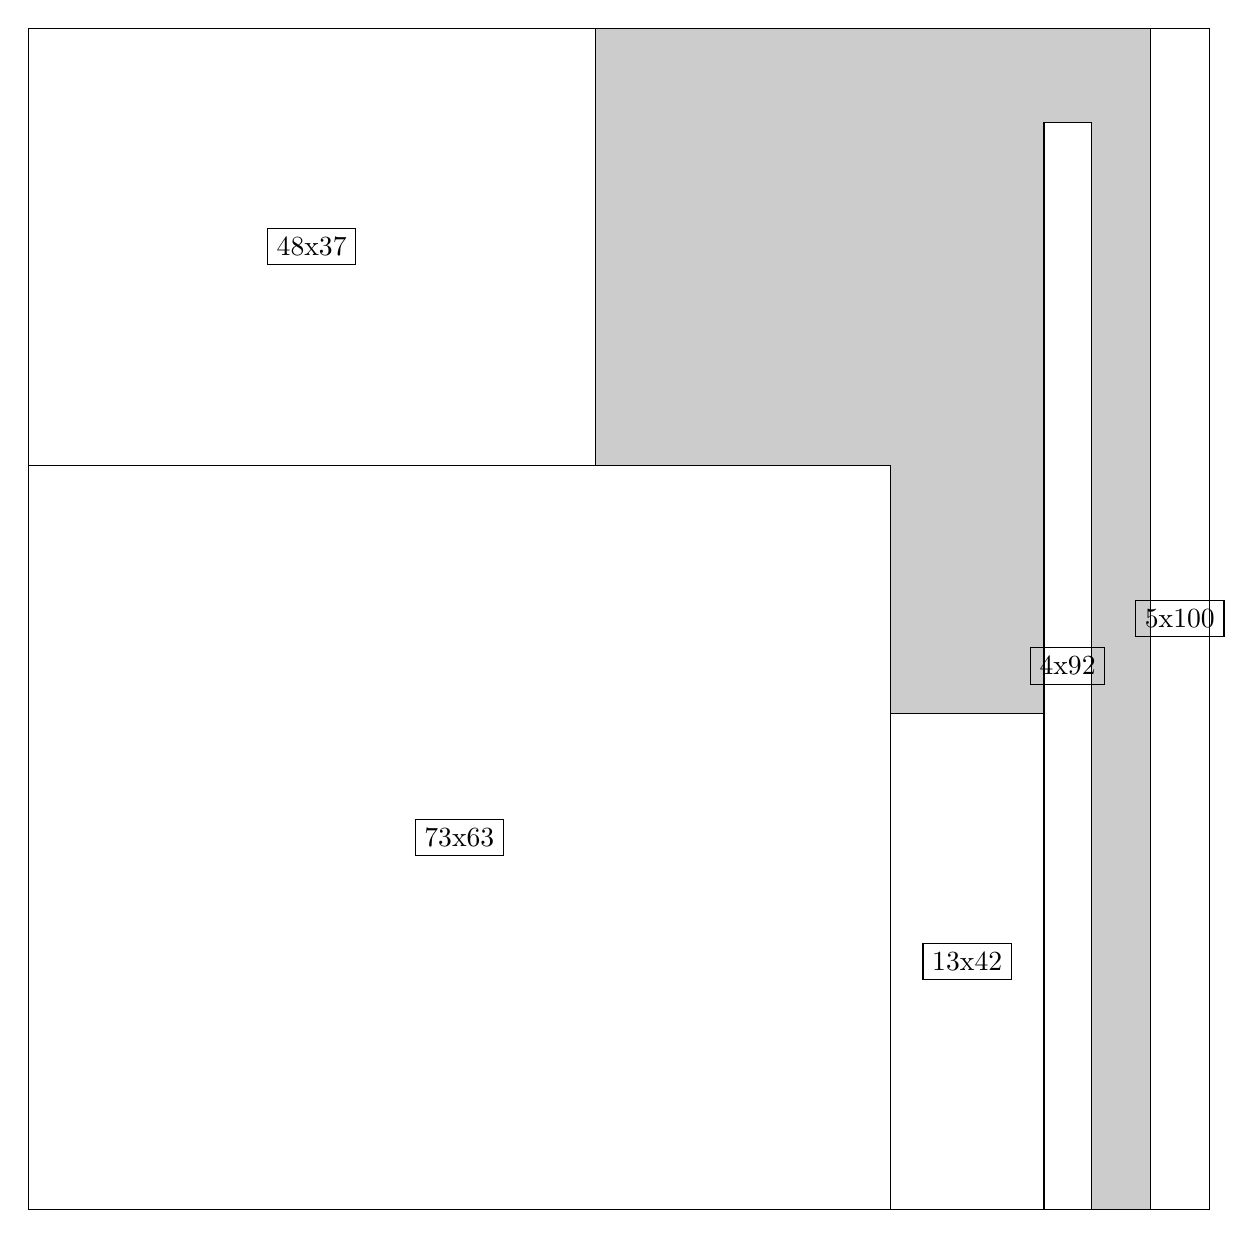
\begin{tikzpicture}[shorten >=1pt,scale=1.0,every node/.style={scale=1.0},->]
\tikzstyle{vertex}=[circle,fill=black!25,minimum size=14pt,inner sep=0pt]
\filldraw[fill=gray!40!white, draw=black] (0,0) rectangle (15.0,15.0);
\foreach \name/\x/\y/\w/\h in {73x63/0.0/0.0/10.95/9.45,48x37/0.0/9.45/7.199999999999999/5.55,13x42/10.95/0.0/1.95/6.3,5x100/14.25/0.0/0.75/15.0,4x92/12.9/0.0/0.6/13.799999999999999}
\filldraw[fill=white!40!white, draw=black] (\x,\y) rectangle node[draw] (\name) {\name} ++(\w,\h);
\end{tikzpicture}


w =73 , h =63 , x =0 , y =0 , v =4599
\par
w =48 , h =37 , x =0 , y =63 , v =1776
\par
w =13 , h =42 , x =73 , y =0 , v =546
\par
w =5 , h =100 , x =95 , y =0 , v =500
\par
w =4 , h =92 , x =86 , y =0 , v =368
\par
\newpage


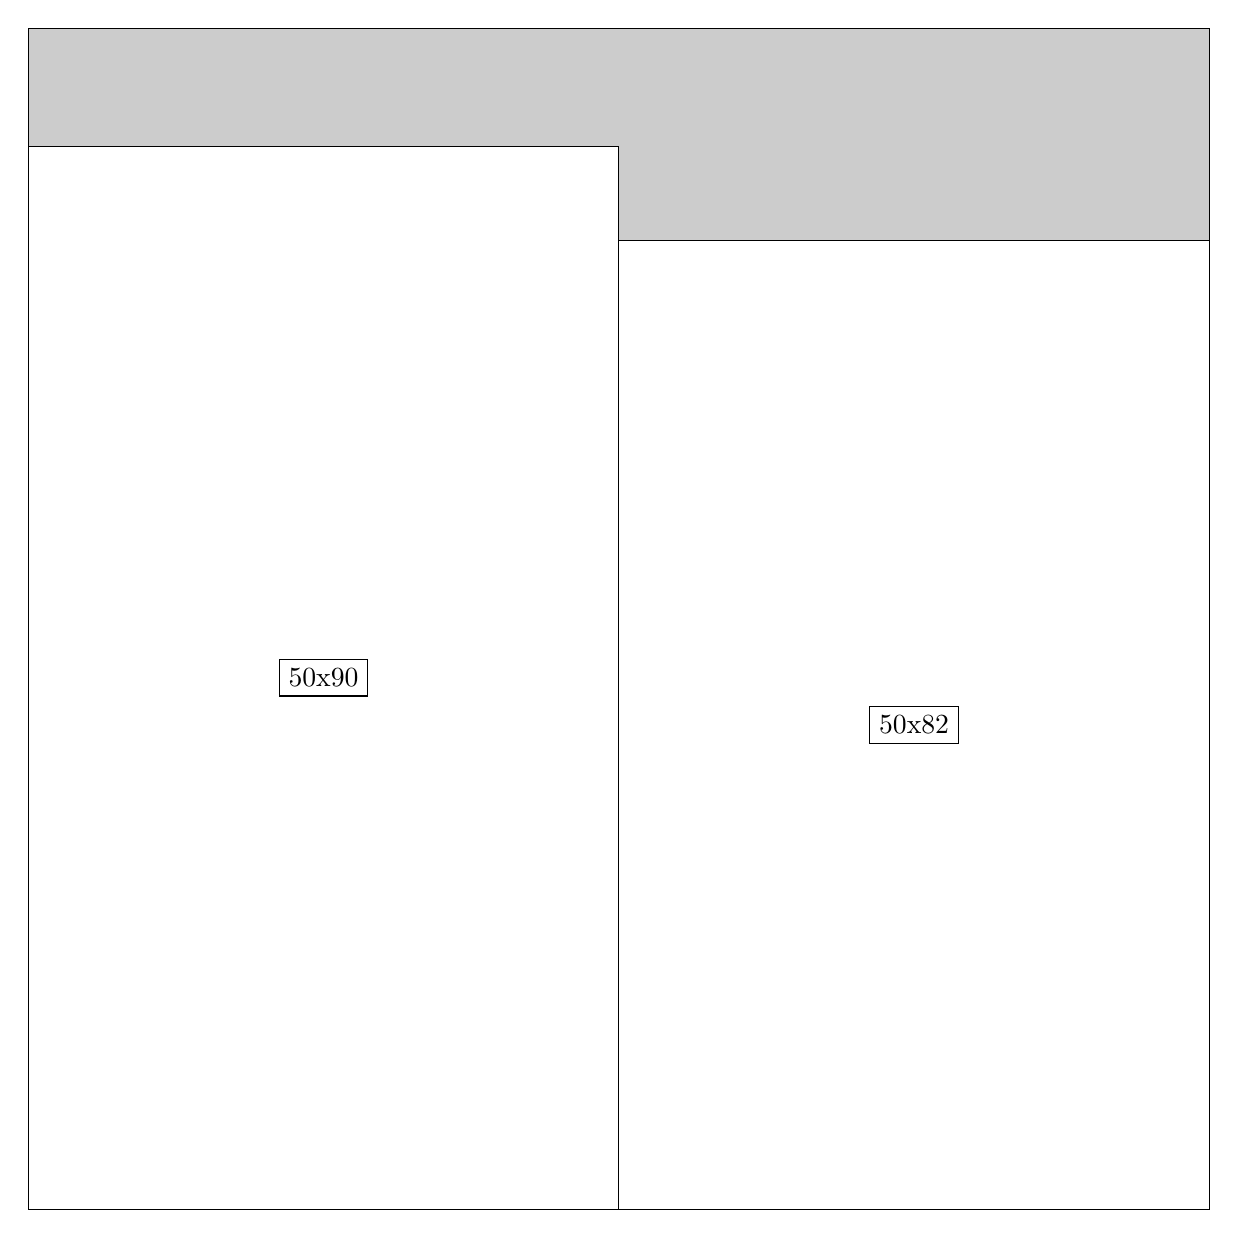
\begin{tikzpicture}[shorten >=1pt,scale=1.0,every node/.style={scale=1.0},->]
\tikzstyle{vertex}=[circle,fill=black!25,minimum size=14pt,inner sep=0pt]
\filldraw[fill=gray!40!white, draw=black] (0,0) rectangle (15.0,15.0);
\foreach \name/\x/\y/\w/\h in {50x90/0.0/0.0/7.5/13.5,50x82/7.5/0.0/7.5/12.299999999999999}
\filldraw[fill=white!40!white, draw=black] (\x,\y) rectangle node[draw] (\name) {\name} ++(\w,\h);
\end{tikzpicture}


w =50 , h =90 , x =0 , y =0 , v =4500
\par
w =50 , h =82 , x =50 , y =0 , v =4100
\par
\newpage


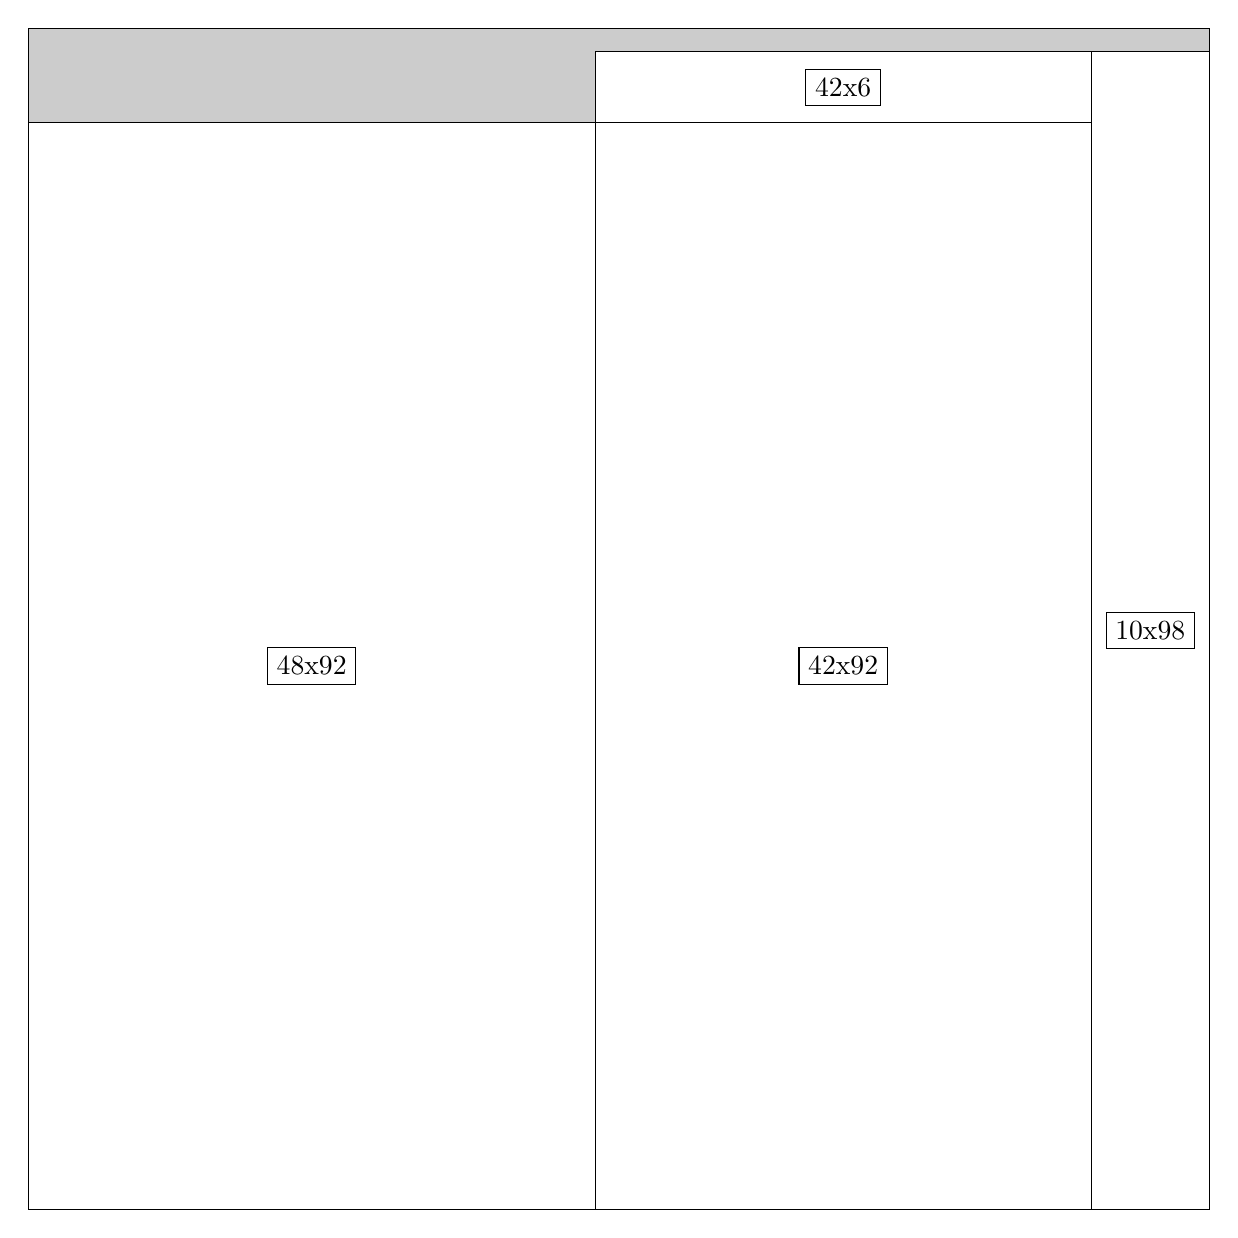
\begin{tikzpicture}[shorten >=1pt,scale=1.0,every node/.style={scale=1.0},->]
\tikzstyle{vertex}=[circle,fill=black!25,minimum size=14pt,inner sep=0pt]
\filldraw[fill=gray!40!white, draw=black] (0,0) rectangle (15.0,15.0);
\foreach \name/\x/\y/\w/\h in {48x92/0.0/0.0/7.199999999999999/13.799999999999999,42x92/7.199999999999999/0.0/6.3/13.799999999999999,10x98/13.5/0.0/1.5/14.7,42x6/7.199999999999999/13.799999999999999/6.3/0.8999999999999999}
\filldraw[fill=white!40!white, draw=black] (\x,\y) rectangle node[draw] (\name) {\name} ++(\w,\h);
\end{tikzpicture}


w =48 , h =92 , x =0 , y =0 , v =4416
\par
w =42 , h =92 , x =48 , y =0 , v =3864
\par
w =10 , h =98 , x =90 , y =0 , v =980
\par
w =42 , h =6 , x =48 , y =92 , v =252
\par
\newpage


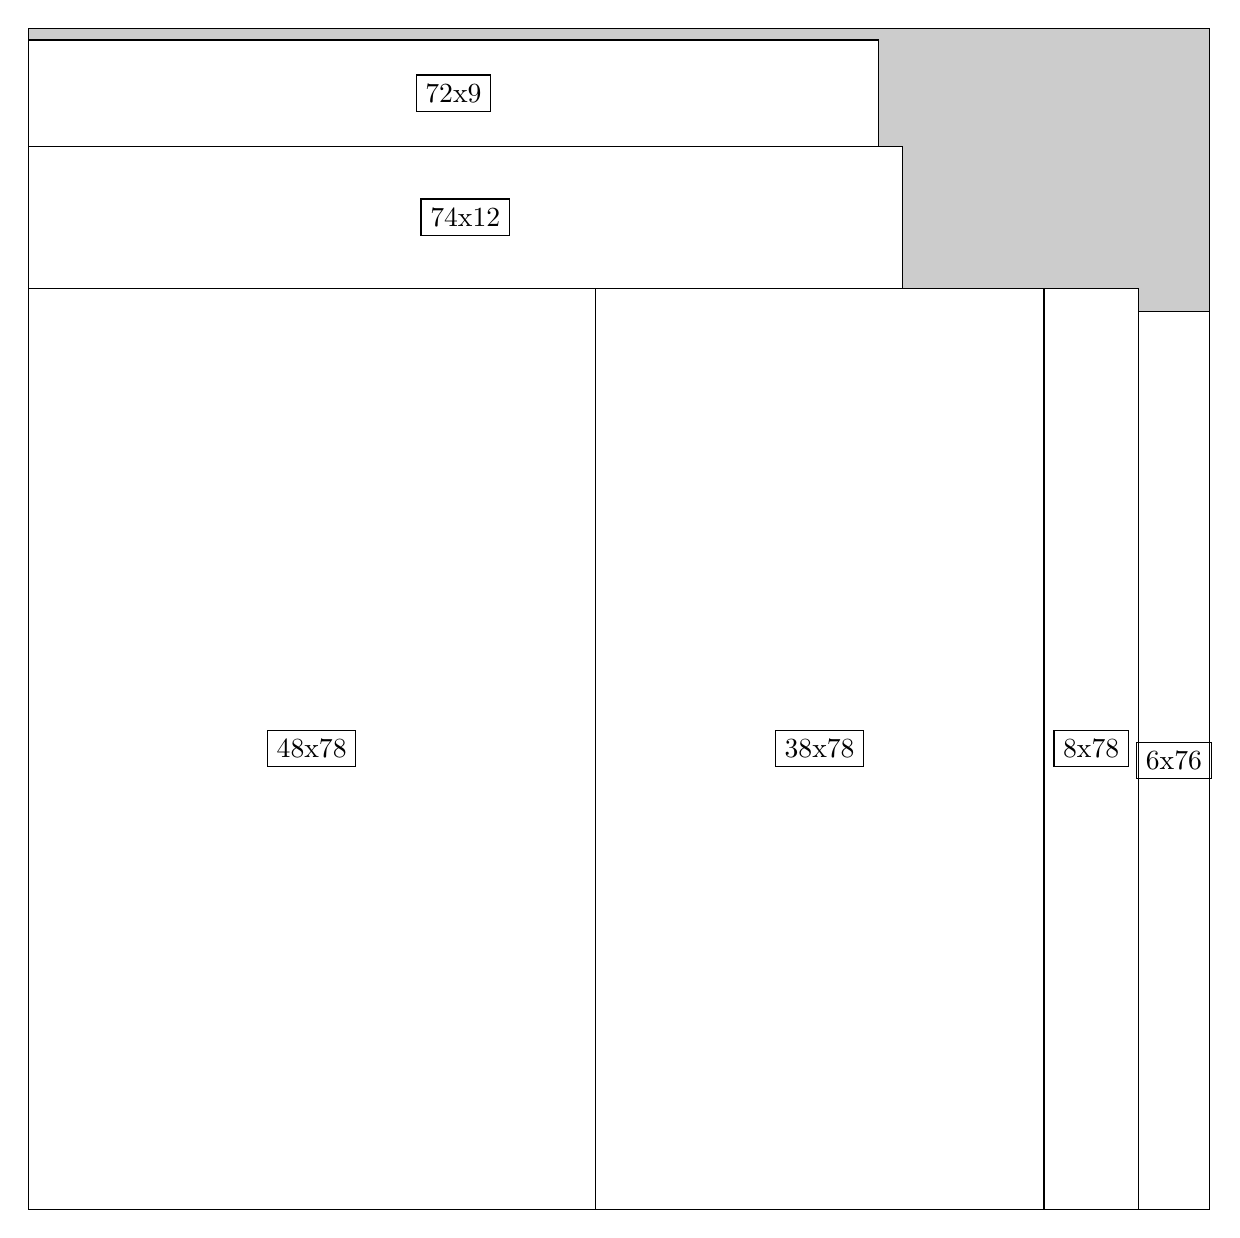
\begin{tikzpicture}[shorten >=1pt,scale=1.0,every node/.style={scale=1.0},->]
\tikzstyle{vertex}=[circle,fill=black!25,minimum size=14pt,inner sep=0pt]
\filldraw[fill=gray!40!white, draw=black] (0,0) rectangle (15.0,15.0);
\foreach \name/\x/\y/\w/\h in {48x78/0.0/0.0/7.199999999999999/11.7,38x78/7.199999999999999/0.0/5.7/11.7,74x12/0.0/11.7/11.1/1.7999999999999998,72x9/0.0/13.5/10.799999999999999/1.3499999999999999,8x78/12.9/0.0/1.2/11.7,6x76/14.1/0.0/0.8999999999999999/11.4}
\filldraw[fill=white!40!white, draw=black] (\x,\y) rectangle node[draw] (\name) {\name} ++(\w,\h);
\end{tikzpicture}


w =48 , h =78 , x =0 , y =0 , v =3744
\par
w =38 , h =78 , x =48 , y =0 , v =2964
\par
w =74 , h =12 , x =0 , y =78 , v =888
\par
w =72 , h =9 , x =0 , y =90 , v =648
\par
w =8 , h =78 , x =86 , y =0 , v =624
\par
w =6 , h =76 , x =94 , y =0 , v =456
\par
\newpage


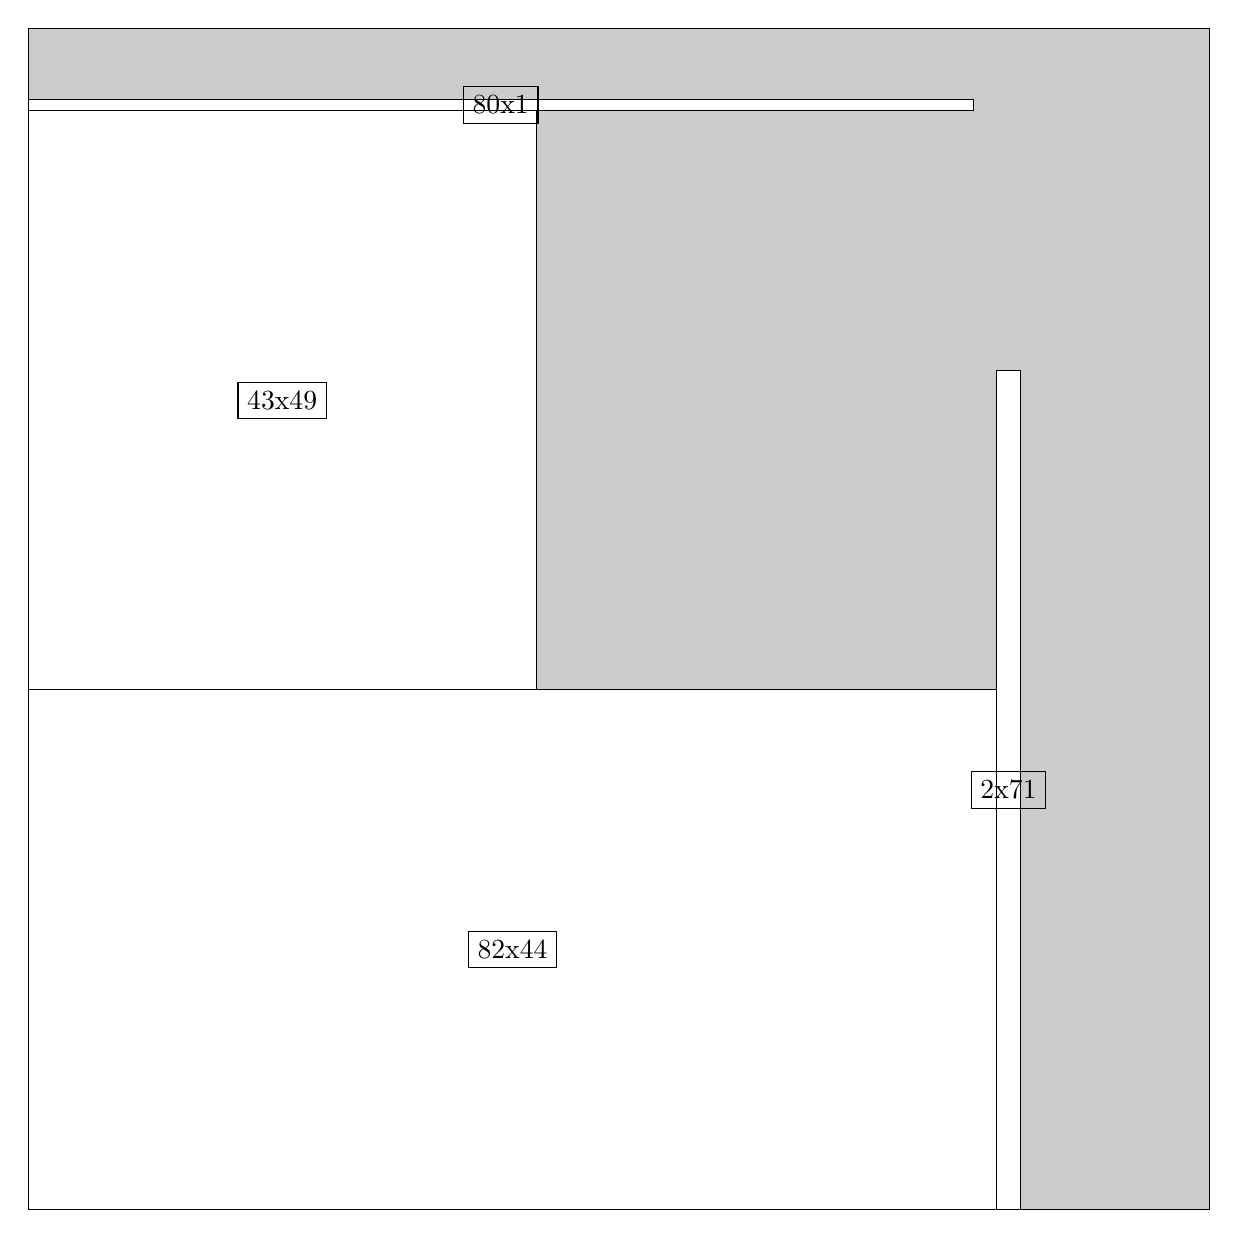
\begin{tikzpicture}[shorten >=1pt,scale=1.0,every node/.style={scale=1.0},->]
\tikzstyle{vertex}=[circle,fill=black!25,minimum size=14pt,inner sep=0pt]
\filldraw[fill=gray!40!white, draw=black] (0,0) rectangle (15.0,15.0);
\foreach \name/\x/\y/\w/\h in {82x44/0.0/0.0/12.299999999999999/6.6,43x49/0.0/6.6/6.45/7.35,80x1/0.0/13.95/12.0/0.15,2x71/12.299999999999999/0.0/0.3/10.65}
\filldraw[fill=white!40!white, draw=black] (\x,\y) rectangle node[draw] (\name) {\name} ++(\w,\h);
\end{tikzpicture}


w =82 , h =44 , x =0 , y =0 , v =3608
\par
w =43 , h =49 , x =0 , y =44 , v =2107
\par
w =80 , h =1 , x =0 , y =93 , v =80
\par
w =2 , h =71 , x =82 , y =0 , v =142
\par
\newpage


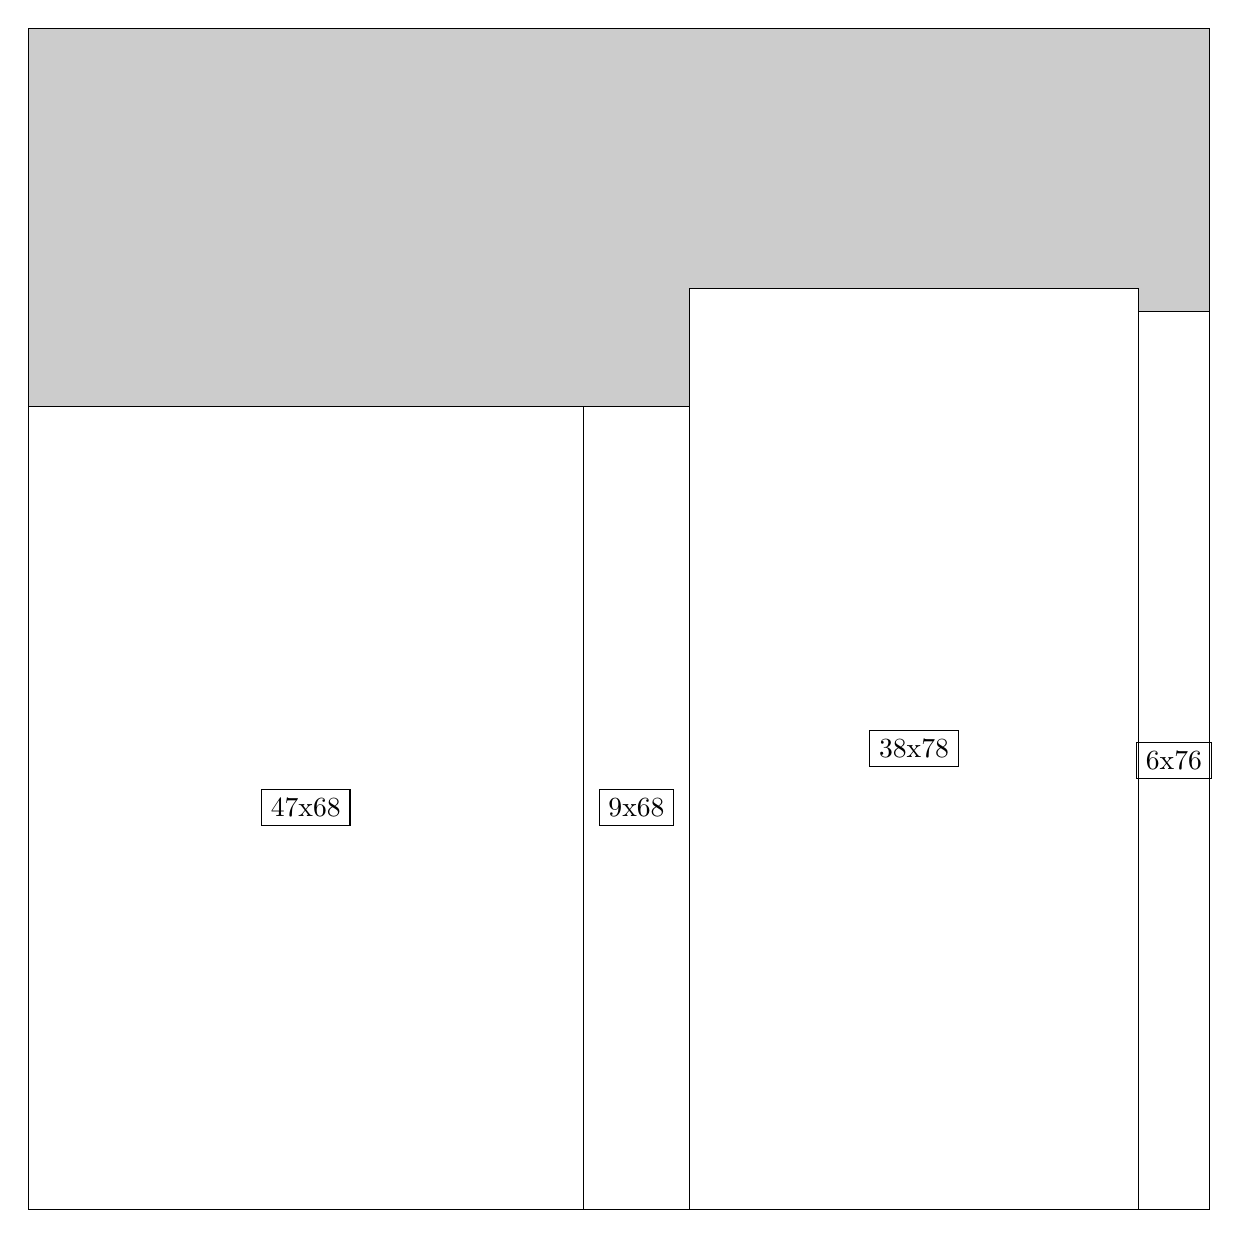
\begin{tikzpicture}[shorten >=1pt,scale=1.0,every node/.style={scale=1.0},->]
\tikzstyle{vertex}=[circle,fill=black!25,minimum size=14pt,inner sep=0pt]
\filldraw[fill=gray!40!white, draw=black] (0,0) rectangle (15.0,15.0);
\foreach \name/\x/\y/\w/\h in {47x68/0.0/0.0/7.05/10.2,38x78/8.4/0.0/5.7/11.7,9x68/7.05/0.0/1.3499999999999999/10.2,6x76/14.1/0.0/0.8999999999999999/11.4}
\filldraw[fill=white!40!white, draw=black] (\x,\y) rectangle node[draw] (\name) {\name} ++(\w,\h);
\end{tikzpicture}


w =47 , h =68 , x =0 , y =0 , v =3196
\par
w =38 , h =78 , x =56 , y =0 , v =2964
\par
w =9 , h =68 , x =47 , y =0 , v =612
\par
w =6 , h =76 , x =94 , y =0 , v =456
\par
\newpage


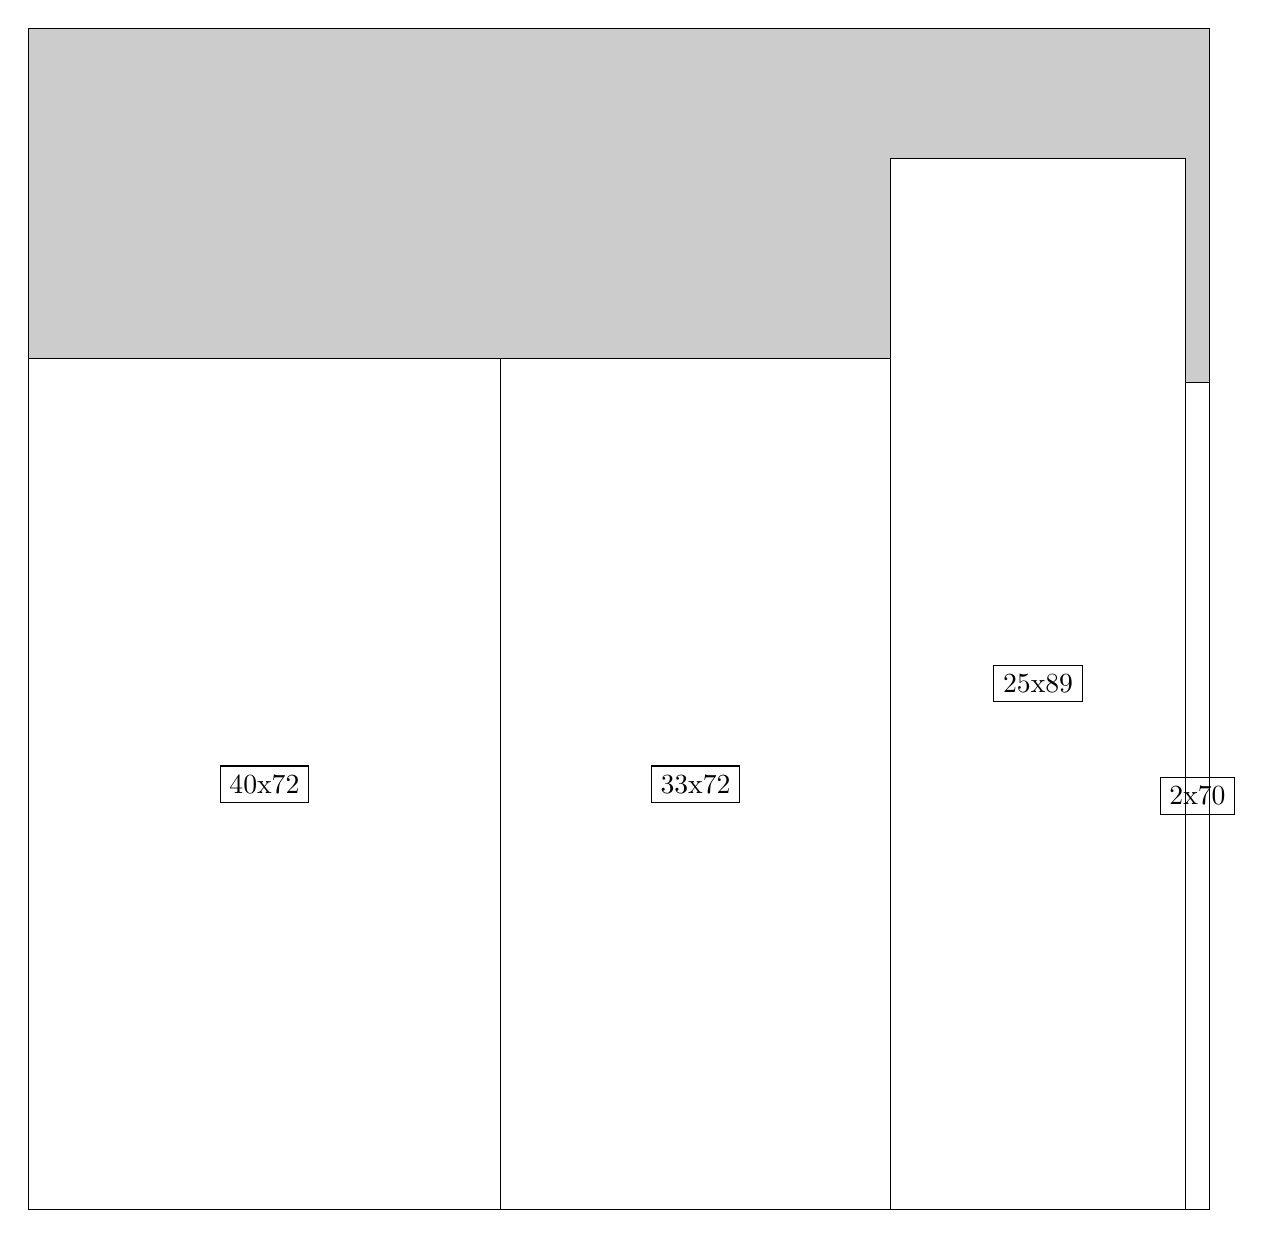
\begin{tikzpicture}[shorten >=1pt,scale=1.0,every node/.style={scale=1.0},->]
\tikzstyle{vertex}=[circle,fill=black!25,minimum size=14pt,inner sep=0pt]
\filldraw[fill=gray!40!white, draw=black] (0,0) rectangle (15.0,15.0);
\foreach \name/\x/\y/\w/\h in {40x72/0.0/0.0/6.0/10.799999999999999,33x72/6.0/0.0/4.95/10.799999999999999,25x89/10.95/0.0/3.75/13.35,2x70/14.7/0.0/0.3/10.5}
\filldraw[fill=white!40!white, draw=black] (\x,\y) rectangle node[draw] (\name) {\name} ++(\w,\h);
\end{tikzpicture}


w =40 , h =72 , x =0 , y =0 , v =2880
\par
w =33 , h =72 , x =40 , y =0 , v =2376
\par
w =25 , h =89 , x =73 , y =0 , v =2225
\par
w =2 , h =70 , x =98 , y =0 , v =140
\par
\newpage


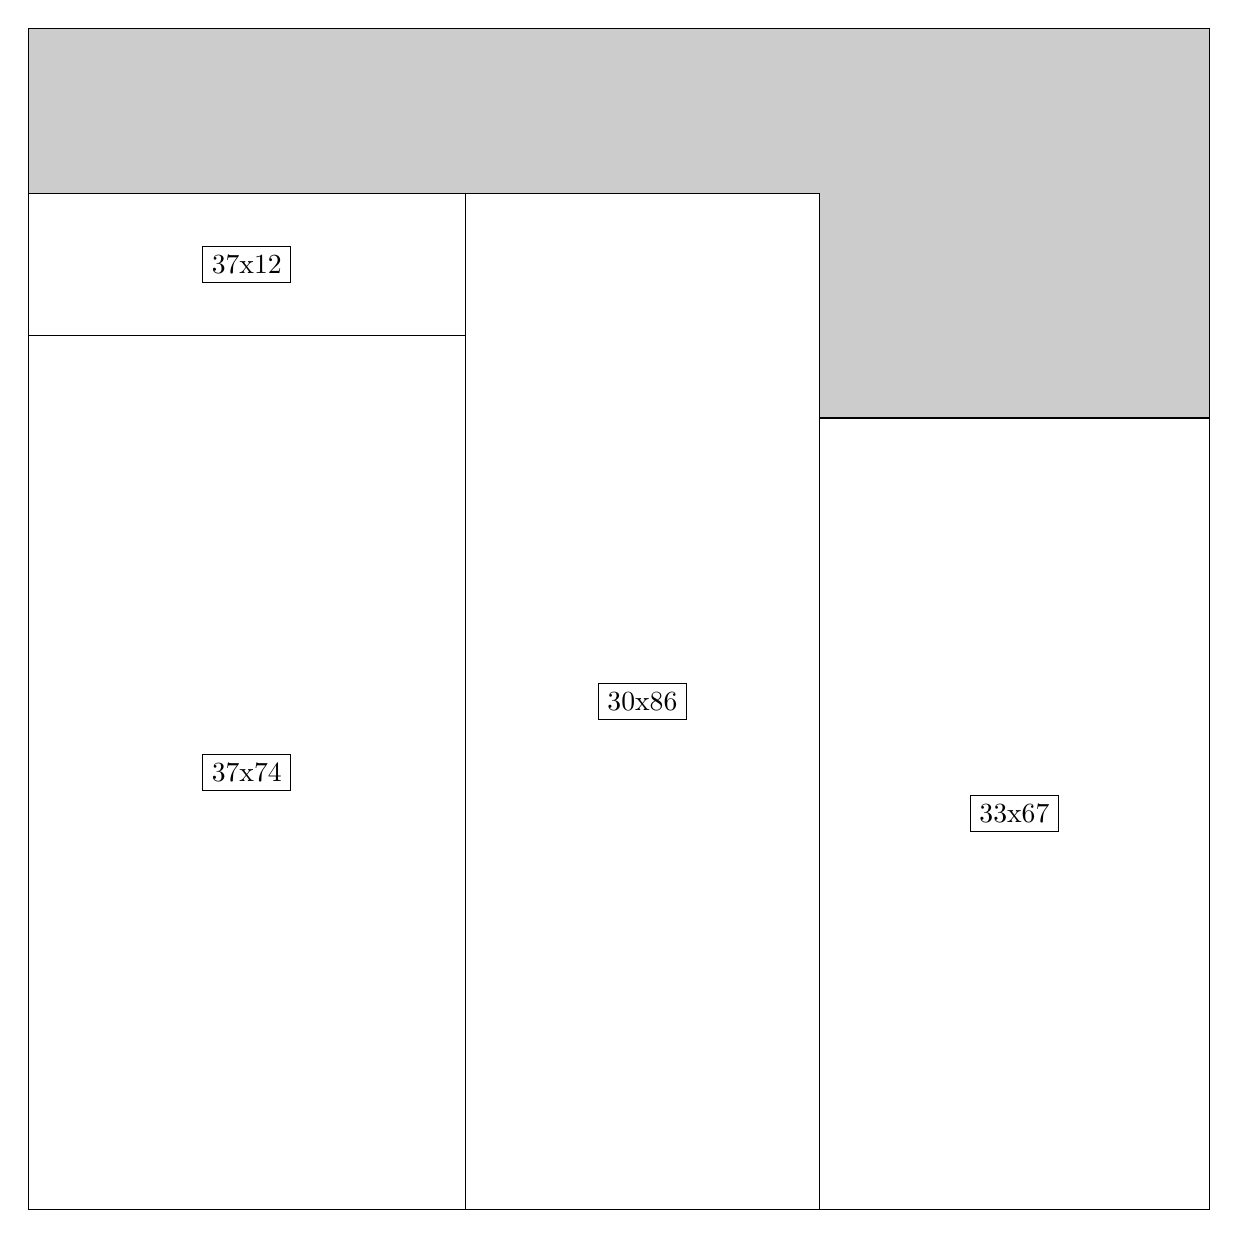
\begin{tikzpicture}[shorten >=1pt,scale=1.0,every node/.style={scale=1.0},->]
\tikzstyle{vertex}=[circle,fill=black!25,minimum size=14pt,inner sep=0pt]
\filldraw[fill=gray!40!white, draw=black] (0,0) rectangle (15.0,15.0);
\foreach \name/\x/\y/\w/\h in {37x74/0.0/0.0/5.55/11.1,30x86/5.55/0.0/4.5/12.9,33x67/10.049999999999999/0.0/4.95/10.049999999999999,37x12/0.0/11.1/5.55/1.7999999999999998}
\filldraw[fill=white!40!white, draw=black] (\x,\y) rectangle node[draw] (\name) {\name} ++(\w,\h);
\end{tikzpicture}


w =37 , h =74 , x =0 , y =0 , v =2738
\par
w =30 , h =86 , x =37 , y =0 , v =2580
\par
w =33 , h =67 , x =67 , y =0 , v =2211
\par
w =37 , h =12 , x =0 , y =74 , v =444
\par
\newpage


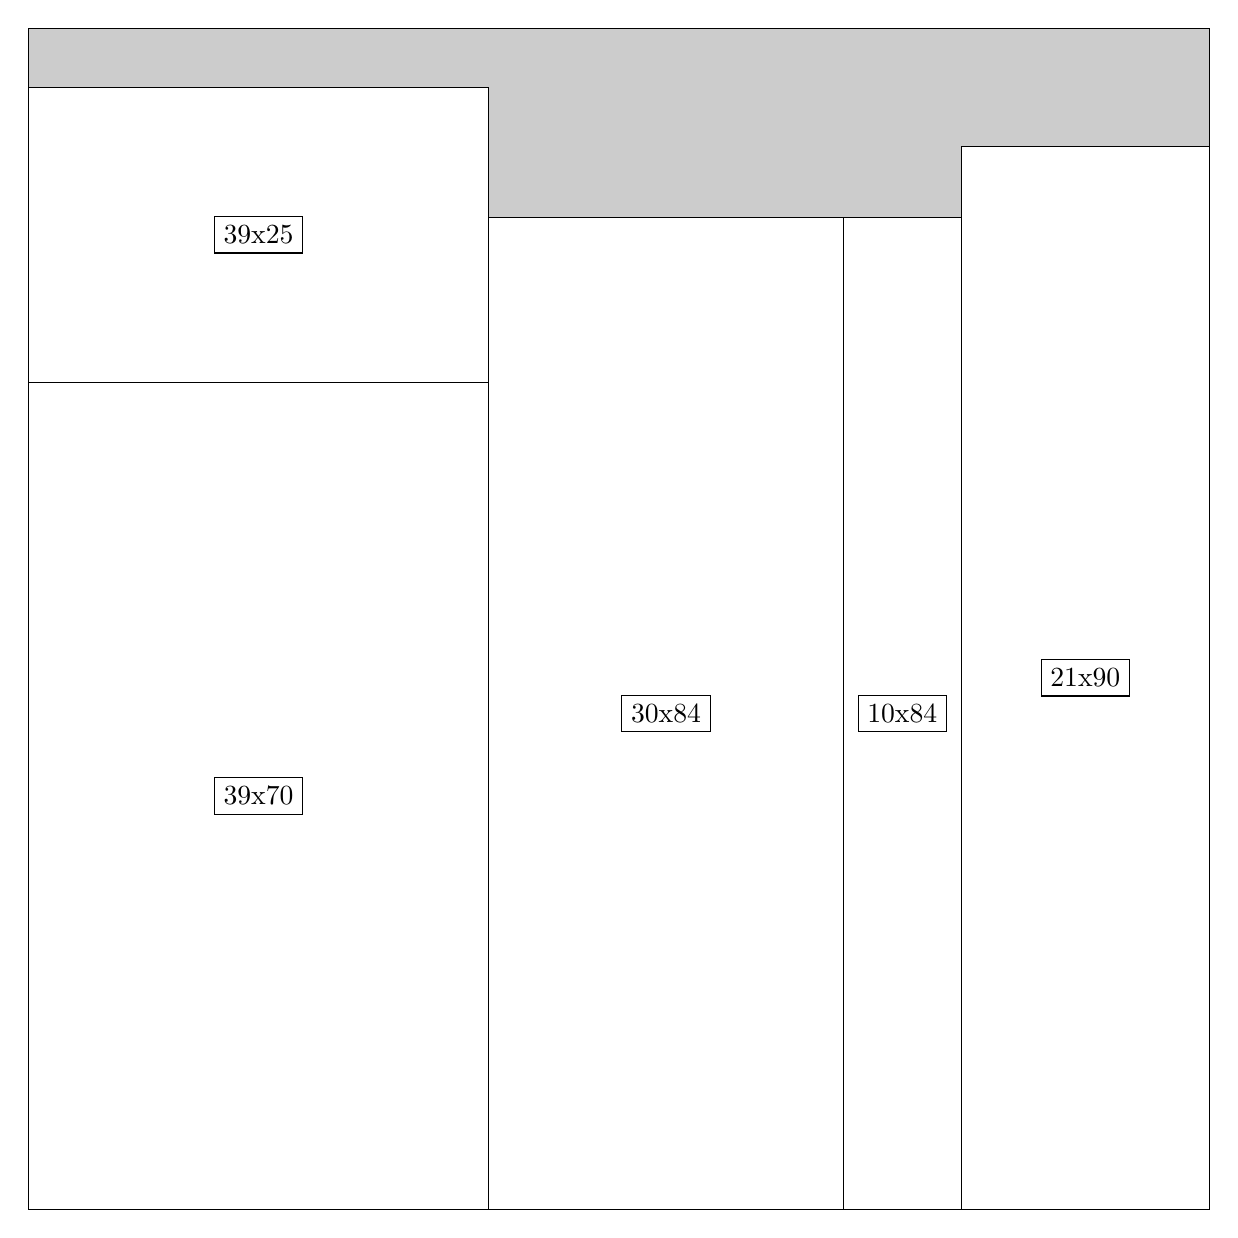
\begin{tikzpicture}[shorten >=1pt,scale=1.0,every node/.style={scale=1.0},->]
\tikzstyle{vertex}=[circle,fill=black!25,minimum size=14pt,inner sep=0pt]
\filldraw[fill=gray!40!white, draw=black] (0,0) rectangle (15.0,15.0);
\foreach \name/\x/\y/\w/\h in {39x70/0.0/0.0/5.85/10.5,30x84/5.85/0.0/4.5/12.6,21x90/11.85/0.0/3.15/13.5,39x25/0.0/10.5/5.85/3.75,10x84/10.35/0.0/1.5/12.6}
\filldraw[fill=white!40!white, draw=black] (\x,\y) rectangle node[draw] (\name) {\name} ++(\w,\h);
\end{tikzpicture}


w =39 , h =70 , x =0 , y =0 , v =2730
\par
w =30 , h =84 , x =39 , y =0 , v =2520
\par
w =21 , h =90 , x =79 , y =0 , v =1890
\par
w =39 , h =25 , x =0 , y =70 , v =975
\par
w =10 , h =84 , x =69 , y =0 , v =840
\par
\newpage


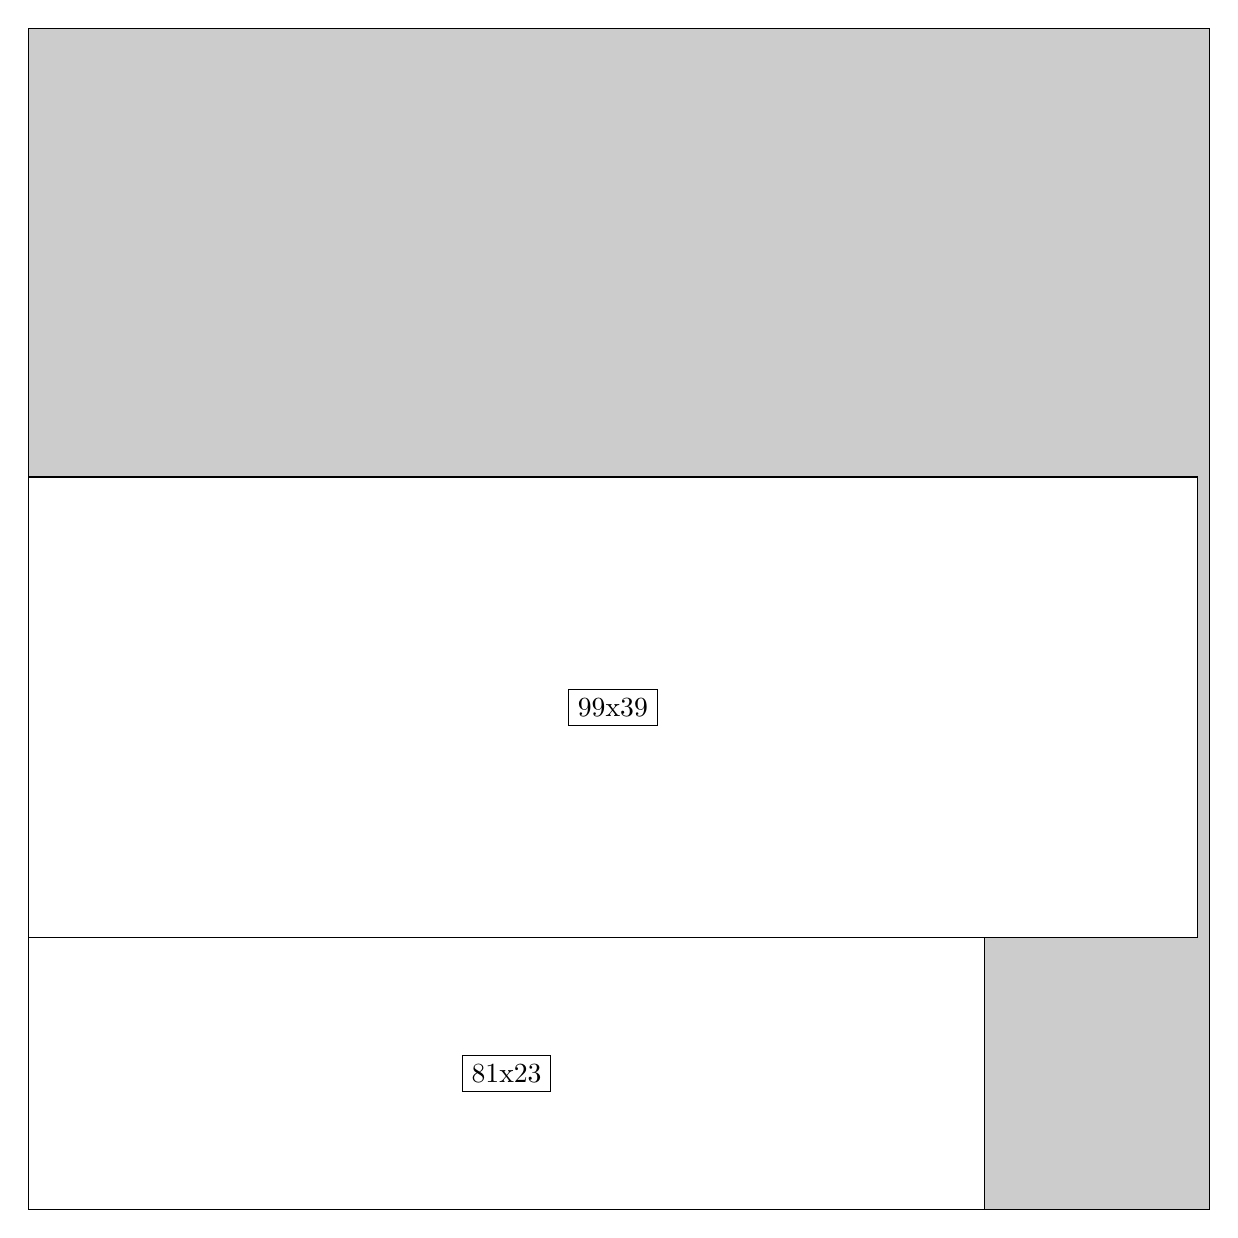
\begin{tikzpicture}[shorten >=1pt,scale=1.0,every node/.style={scale=1.0},->]
\tikzstyle{vertex}=[circle,fill=black!25,minimum size=14pt,inner sep=0pt]
\filldraw[fill=gray!40!white, draw=black] (0,0) rectangle (15.0,15.0);
\foreach \name/\x/\y/\w/\h in {99x39/0.0/3.4499999999999997/14.85/5.85,81x23/0.0/0.0/12.15/3.4499999999999997}
\filldraw[fill=white!40!white, draw=black] (\x,\y) rectangle node[draw] (\name) {\name} ++(\w,\h);
\end{tikzpicture}


w =99 , h =39 , x =0 , y =23 , v =3861
\par
w =81 , h =23 , x =0 , y =0 , v =1863
\par
\newpage


\end{document}